Tendo em vista que o balão necessitará armazenar informações das filmagens, apresentar as informações, tanto em tempo real, quanto sob demanda, será necessário um desenvolvimento de um software próprio para que suporte algumas características do projeto.

\subsection{Visão geral do produto}

O software em questão será subdividido em duas partes, o software que estará no balão, embarcado, e o software que estará em terra, central de controle.

\subsubsection{Software embarcado}

O software embarcado irá se basear em apenas recolher os dados dos sensores e câmeras e enviar para a central de controle.

O envio dos dados será realizado utilizando um serviço \textit{restfull} para simplificar e reduzir os custos e o peso de hardware no balão, deixando a responsabilidade de processar, catalogar e armazenar os dados enviados com o lado servidor que se encontrará em terra.

\subsubsection{Central de controle}

O software que estará em terra será o responsável por recolher os dados enviados pelo software embarcado e armazenar essas informações no banco de dados, alem de ser responsável pela redundância de dados e resiliência do sistema como um todo, evitando assim falhas previstas e tornando possível um maior tempo de operação direta.

\subsubsection{Resumo das capacidades}

Nesta seção serão descritos o que será delegado a cada parte do software e o que está dentro ou fora das capacidades do mesmo.

\paragraph{Software embarcado}

O software embarcado será responsável pelo recolhimento dos dados de cada sensor, compilando-os em uma pacote para que este possa ser enviado ao servidor, devendo ser capaz de identificar se o serviço ao qual irá consumir está disponível, e caso não esteja possa salvar as informações durante um curto período de tempo e enviar ao servidor quando o serviço estiver novamente funcional.

Além da capacidade de perceber se o serviço está funcional ou não, o software embarcado deve ser capaz de verificar um mal funcionamento em algum sensor do balão para que as devidas providências possam ser tomadas.

\paragraph{Central de controle}

O software em terra será o coração do controle informatizado, sendo responsável por servir o software embarcado com um serviço \textit{restfull} para possibilitar a comunicação rápida e direta entre as duas partes.

Além do serviço, a central de controle será responsável pela redundância de dados para segurança da informação e detecção de falhas para ter a possibilidade de correção automática.

\subsection{Requisitos}

Os requisitos do software são informações das quais serão levantados caso de uso para o sistema, que por sua vez nortearão o desenvolvimento das funcionalidades delimitando o que cada uma deve ou não conter.

\begin{itemize}
  \item O sistema deve ser capaz de interfaciar com diversos sensores, sendo capaz de incluir novos caso haja a necessidade.
  \item O sistema deve realizar um \textit{backup} das informações dos vídeos a cada 2 horas.
  \item O sistema deve ser capaz de identificar mal funcionamento nos sensores aos quais estabelece interface.
  \item O sistema deve avisar quando forem detectados falhas ou mal funcionamento tanto na unidade terrestre quanto na unidade aérea.
\end{itemize}

Os requisitos do Software presente na Central de Controle foram obtidos a partir de uma técnica de obtenção de requisitos de forma Tradicional, especificando o Problema a ser solucionado, as Necessidades encontradas, suas características e os Casos de Uso do Sistema.

\subsubsection{O Problema}

	O problema a ser solucionado se refere a questão de segurança no Estacionamento do Campus Gama da Universidade de Brasília. Muitos quesitos levam a ocorrência deste problema, como o baixo volume de circulação de pessoas, a ausência de câmeras, a localização isolada e até a falta de segurança nos próprios carros dos frequentadores da Universidade.

	Para melhor entendimento do problema em questão, utilizou-se da técnica de \textit{Framework de ishikawa}, também conhecido como \textit{Fishbone}. A figura \ref{img:fishbone} apresenta o Problema a ser solucionado.

	\begin{figure}[H]
		\centering
		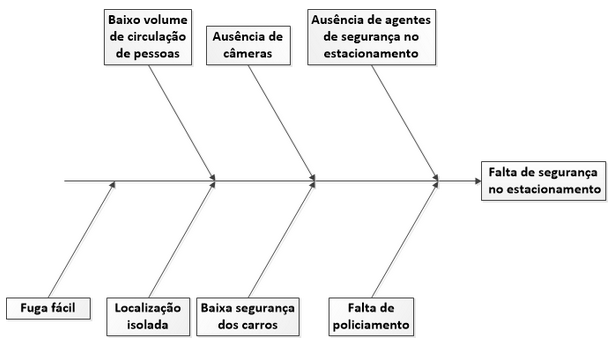
\includegraphics[width=0.9\textwidth]{figuras/fishbone}
		\caption{Diagrama de \textit{Ishikawa} }
		\label{img:fishbone}
	\end{figure}

	Outra técnica bastante utilizada pelo mercado da Engenharia de Software para o entendimento do Problema, é a utilização do Framework de Problema, o qual está presente a seguir.

	\begin{table}[H]
		\centering
		\label{my-label}
		\begin{tabular}{lllll}
			\cline{1-2}
			\multicolumn{1}{|l|}{\textbf{O Problema de}}                      & \multicolumn{1}{l|}{Segurança no estacionamento da UnB Gama.}                                                                                                                  & \textbf{} & \textbf{} & \textbf{} \\ \cline{1-2}
			\multicolumn{1}{|l|}{\textbf{Afeta}}                              & \multicolumn{1}{l|}{\begin{tabular}[c]{@{}l@{}}Alunos, professores, servidores e pessoas que \\ utilizam deste espaço.\end{tabular}}                                           &           &           &           \\ \cline{1-2}
			\multicolumn{1}{|l|}{\textbf{Cujo Impacto é}}                     & \multicolumn{1}{l|}{Insegurança, roubos.}                                                                                                                                      &           &           &           \\ \cline{1-2}
			\multicolumn{1}{|l|}{\textbf{Uma solução bem sucedida incluiria}} & \multicolumn{1}{l|}{\begin{tabular}[c]{@{}l@{}}Utilização de um dispositivo que permitisse aos \\ interessados monitorar o estacionamento do \\ campus UnB Gama.\end{tabular}} &           &           &           \\ \cline{1-2}

		\end{tabular}
		\caption{Framework do Problema}
	\end{table}

	Após o entendimento do problema, vê-se necessária a documentação das necessidades. Utilizou-se
uma técnica chamada \textit{framework de necessidades} na qual são apresentados todos os problemas, as necessidades, a solução atual e a solução proposta. Dessa forma, pode-se obter um entendimento mais organizado dos problemas as necessidades, de acordo com o retratado na tabela abaixo.

	\begin{table}[H]
		\centering
		\label{tab:necessidades}
		\begin{tabular}{|l|l|l|l|}
			\hline
			\textbf{Necessidade}                                                                              & \textbf{Problema}                                                                 & \textbf{Solução Atual}                                                    & \textbf{Solução Proposta}                                                                                                                      \\ \hline
			\begin{tabular}[c]{@{}l@{}}Observar a situação \\ do estacionamento \\ em tempo real\end{tabular} & \begin{tabular}[c]{@{}l@{}}Baixo volume de \\ circulação de pessoas.\end{tabular} & \begin{tabular}[c]{@{}l@{}}Rondas raras da\\ Polícia Militar\end{tabular} & \begin{tabular}[c]{@{}l@{}}Prover uma filmagem de \\ todo o estacionamento,\\ apresentando as imagens, \\ ao vivo, pela internet.\end{tabular} \\ \hline
			\begin{tabular}[c]{@{}l@{}}Identificar \\ criminosos\end{tabular}                                 & Fuga fácil                                                                        & Sem solução.                                                              & \begin{tabular}[c]{@{}l@{}}Com filmagens, a \\ identificação se torna \\ viável.\end{tabular}                                                  \\ \hline
			\begin{tabular}[c]{@{}l@{}}Informar a Polícia \\ em casos de roubos\end{tabular}                  & Falta de policiamento                                                             & Sem solução.                                                              & \begin{tabular}[c]{@{}l@{}}Os usuários poderão, a partir \\ da visualização das imagens, \\ contactar a PM do Gama.\end{tabular}               \\ \hline
		\end{tabular}
		\caption{Framework de Necessidades}
	\end{table}